We consider the stationary Gaussian RF $\{r(\vect{x}) \ssep \vect{x} \in \mathrm{D} \subset \R^2\}$ with $\mathrm{D} \colon [(1,30), (1,30)]$,
%
\begin{align*}
    \E\{r(\vect{x})\} &= \mu_r = 0 \\
    \Var\{r(\vect{x})\} &= \sigma_r^2 \\
    \Corr\{r(\vect{x}), r(\vect{x'})\} &= \exp\{-\tau/\xi_r\}
\end{align*}
%
and $\tau = |\vect{x} - \vect{x'}|$.

%%%%%%%%%%%%%%%%%%%%%%%%%%%%%%%%%%%%%%%%%%%%%%%%%%%%%%%%%%%%%%%%%%%%%%
\paragraph{a)}
We consider the discretized Gaussian RF $\{r(\vect{x}) \ssep \vect{x} \in \mathrm{L}\}$ on the grid $\mathrm{L} \colon [30 \times 30] \in \mathrm{D}$ with model parameters $\sigma_r^2=2$ and $\xi_r=15$. In figure~\ref{fig:3a_realization} we see one realization of the discretized Gaussian RF.

\begin{figure}
    \centering
    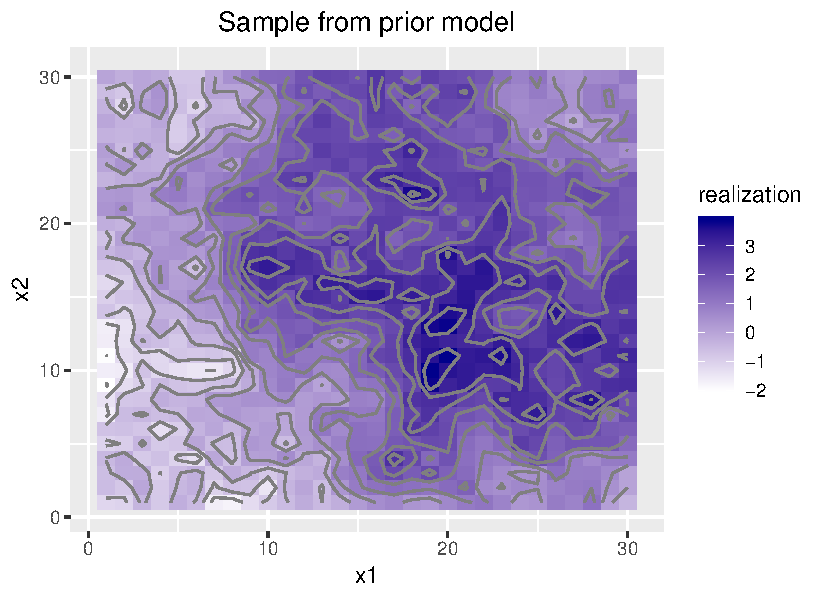
\includegraphics[scale=0.95]{figures/3a_realization.pdf}
    \caption{One realization of the discretized Gaussian RF given in \ref{sec:problem3}a.}
    \label{fig:3a_realization}
\end{figure}

%%%%%%%%%%%%%%%%%%%%%%%%%%%%%%%%%%%%%%%%%%%%%%%%%%%%%%%%%%%%%%%%%%%%%%
\paragraph{b)}
The variogram function for the Gaussian RF is
%
\begin{align*}
\gamma_r(\tau)
\coloneqq&\: \frac{1}{2} \Var \{ r(x) - r(x') \} \\
=&\: \sigma_r^2 - \Cov\{r(x), r(x')\} \\
=&\: \sigma_r^2 - \exp\{-\tau/\xi_r\} \, .
\end{align*}
%
This is shown in figure~\ref{fig:3b_variogram} together with the empirical variogram based on exact observations of the full realization in a). \textcolor{red}{Comment + caption}  

\begin{figure}
    \centering
    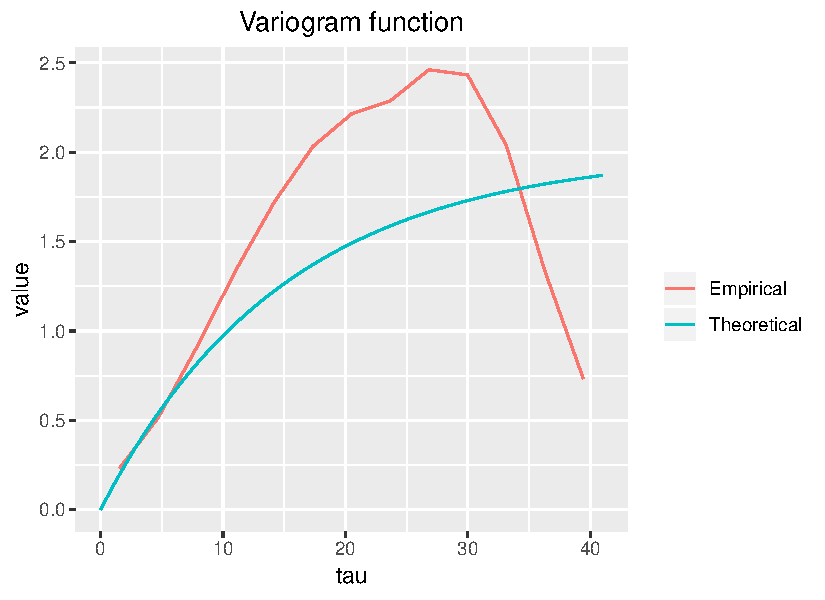
\includegraphics[scale=0.95]{figures/3b_variogram.pdf}
    \caption{!!!One realization of the discretized Gaussian RF given in \ref{sec:problem3}a.}
    \label{fig:3a_realization}
\end{figure}

%%%%%%%%%%%%%%%%%%%%%%%%%%%%%%%%%%%%%%%%%%%%%%%%%%%%%%%%%%%%%%%%%%%%%%
\paragraph{c)}
text text text

%%%%%%%%%%%%%%%%%%%%%%%%%%%%%%%%%%%%%%%%%%%%%%%%%%%%%%%%%%%%%%%%%%%%%%
\paragraph{d)}
text text text

%%%%%%%%%%%%%%%%%%%%%%%%%%%%%%%%%%%%%%%%%%%%%%%%%%%%%%%%%%%%%%%%%%%%%%
\paragraph{e)}
text text text
